\chapter{Edge Offloading \& Early Exiting}

In this chapter we implement a edge-based offloading scheme utilizing early exiting \gls{dnn}s. Our scheme a more flexible and adaptive than currently proposed in literature. In section \ref{} we present our offloading scheme and implementation details. In section \ref{label} we define the system model used to evaluate our result. In section \ref{} we describe our experimental setup. In section \ref{} we present our results and in section \ref{} we discuss our results.

\section{Do we have a catchy name for offloading scheme?}

We propose a more flexible edge offloading scheme compared to Edgent \cite{li_edge_2018}. Edgent is to our knowledge the only proposal in current literature, that uses early exiting models in an offloading scenario. Edgent combines early exiting and network splitting to handle the accuracy-latency trade-off, by an optimization framework of \gls{dnn} right-sizing and splitting for device-edge collaboration. The optimization done based on regression models of the per layer execution time of the \gls{dnn}. The downside of edgent is an upfront selection of exit i.e gls{dnn} right-sizing, which can be troublesome with unpredictable communication delays. 

We argue, that allowing the edge server to reach as far as possible, within the time budget and continuously sending back increasingly confident predictions, will in any case achieve at least the same accuracy. Even though a sub-model exit have been chosen with care e.g. using \gls{dnn} right-sizing, the risk of timeout is still present as both computation and communication delays are not constant. If unexpected delays do occur, it may cause timeouts and lead to lost predictions. However, our scheme reduces the risk of losing prediction by timeout, if an earlier, albeit less accurate predictions is available. 

Figure \ref{fig:offloading-scheme} illustrates the offloading scheme. To not waste idle time on edge server the data is immediately offloaded from the end device, to edge server. The edge server preprocesses the data, runs the \gls{dnn} inference process, and whenever a prediction is obtained from the early ecit \gls{dnn}, a thread is spawned to send back the result to the end device. Multiple early exits allows for successively receiving, what is expectedly, increasingly reliable predictions. The most recent received prediction i.e. from the latest exits are accepted as the prediction.

We send back the top-5 predictions to allow info-combination and reduce the data size of the reply. We use top-5, since the correct class is within these 5 predictions close to 90 \% of the time having just two predictions available for any of the models, see figure \ref{fig:top-5-cumulative}. The end device then decides the prediction based upon the information received from the edge server. Figure \ref{fig:offloading-scheme-successful} illustrates the continuous reply of predictions. Figure \ref{fig:offloading-scheme-timeout} illustrates a case, where a timeout occurs and only two predictions are available.

\begin{figure}
	\captionsetup[subfigure]{justification=centering}
	\centering
	\subfloat[Continuois predictions\label{fig:offloading-scheme-successful}]{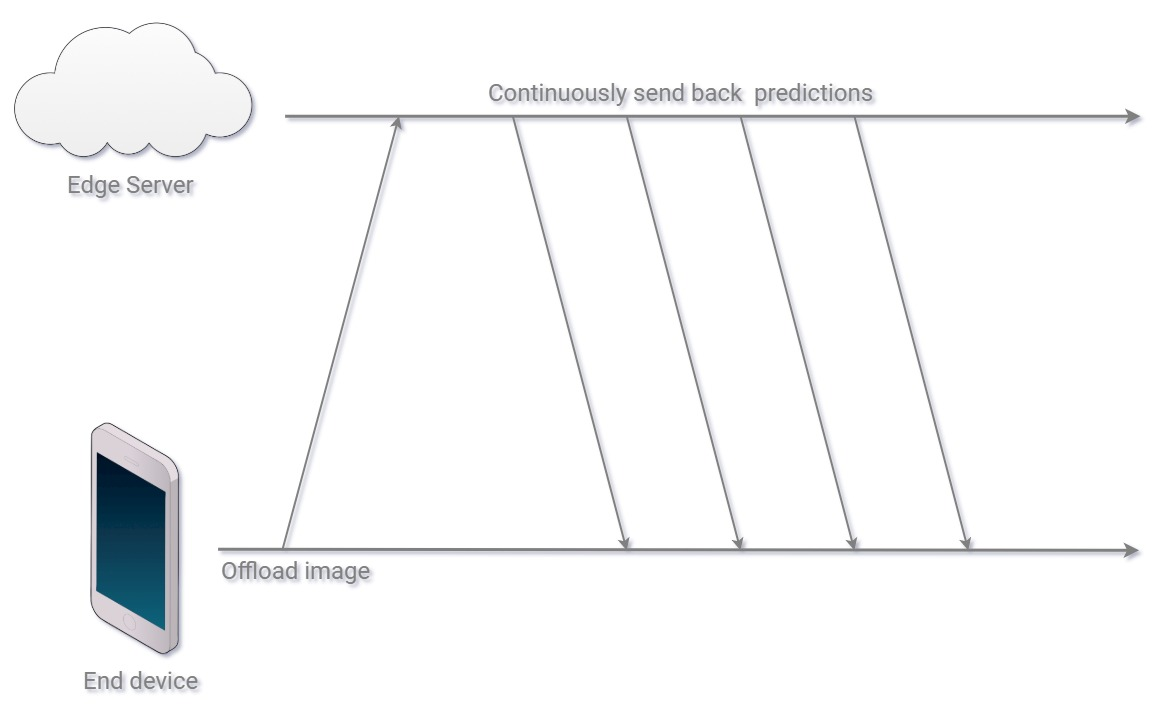
\includegraphics[width=.7\linewidth]{figures/models/timeline_all}}
	\hfill
	\subfloat[Timeout of Continuois predictions\label{fig:offloading-scheme-timeout}]{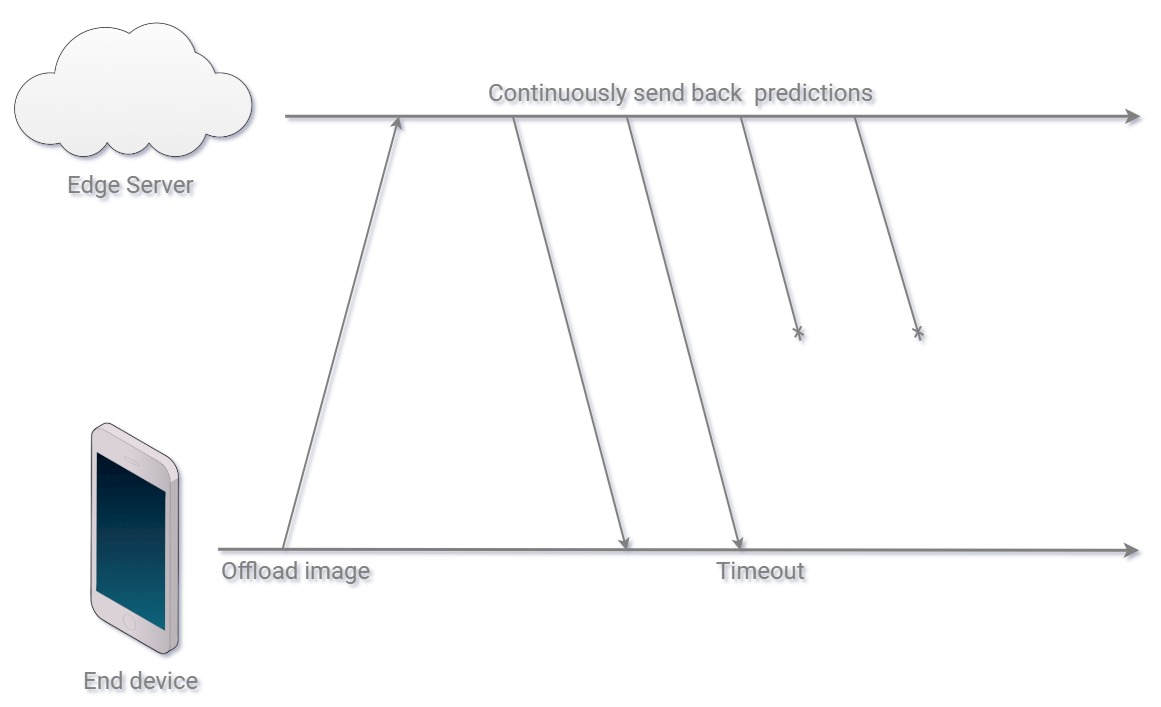
\includegraphics[width=.7\linewidth]{figures/models/timeline_timeout}}
	\caption[Offloading scheme]{offloading scheme}
	\label{fig:offloading-scheme}
\end{figure} 

To combine top-5 prediction information from $ n $ exits, we must expand the vectors back to the original class space of $ C $ dimensions.

Each exit outputs two 5-dimensional vectors. $\mathbf{l}_{i,k}^{top5}$ contains the labels of the top-5 predictions and $ \mathbf{\hat{y}}_{i,k}^{top5}$ contain the class scores of the top-5 predictions. 

\begin{align}
\begin{split}
\mathbf{l}_{i,n}^{top5} &= \begin{bmatrix}
l_{i,n}^{1st} & \phantom{.}l_{i,n}^{2nd} & \phantom{.}l_{i,n}^{3rd} & \phantom{.}l_{i,n}^{4th} & \phantom{.}l_{i,n}^{5th}
\end{bmatrix}, \\
\mathbf{\hat{y}}^{top5}_{i,n} &= \begin{bmatrix}
\hat{y}_{i,n}^{1st} & \hat{y}_{i,n}^{2nd} & \hat{y}_{i,n}^{3rd} & \hat{y}_{i,n}^{4th} & \hat{y}_{i,n}^{5th}
\end{bmatrix}
\end{split}
\end{align}

The vectors are sorted from highest to lowest, hence the score $ \hat{y}_{i,k}^{1st} $ is associated the label $ l_{i,k}^{1st} $ etc. 

We define an expansion function, which takes the top-5 score vector $ \mathbf{\hat{y}}_{i,n}^{top5}$ and top-5 label vector  $\mathbf{l}_{i,n}^{top5}$ as input  $ f_{expand}\left(\bm{\hat{y}}_{i,n}^{top5},\mathbf{l}_{i,n}^{top5}\right) $ and outputs a $ C $-dimensional score vector, with the scores value at corresponding class index of the label vector, with the remaining indices are zero.
\begin{align}
f_{expand}\left(\bm{\hat{y}}_{i,n}^{top5},\mathbf{l}_{i,n}^{top5}\right) = 
\begin{bmatrix}
\hat{y}_{i,n,1} & \hat{y}_{i,n,2} & \hat{y}_{i,n,c} & \dots & \hat{y}_{i,n,C}
\end{bmatrix}_{1 \times C}
\end{align}
\todo{is this implementation?}

\paragraph{Example: Expansion of a 10 class problem} 
\blockquote[]{	 	
	For this classification example, the number of classes $C=10$. From a prediction we get the two output vectors $\mathbf{l}_{i,n}^{top5}$ and $ \mathbf{\hat{y}}_{i,n}^{top5}$.
	\begin{align*}
	\mathbf{l}_{i,n}^{top5} &= \begin{bmatrix}
	\phantom{0}0\phantom{.0} & \phantom{0}3\phantom{.0} & \phantom{0}6\phantom{.0} & \phantom{0}8\phantom{.0} & \phantom{0}9\phantom{.0}
	\end{bmatrix},\\
	\mathbf{\hat{y}}_{i,n}^{top5} &= \begin{bmatrix}
	0.80 & 0.10 & 0.05 & 0.03 & 0.01
	\end{bmatrix}
	\end{align*}
	We use our expansion function $ f_{expand}\left(\bm{\hat{y}}_{i,n}^{top5},\mathbf{l}_{i,n}^{top5}\right) $, which return the score vector $ \mathbf{\hat{y}}_{i,n}$.
	\begin{align*}
	\mathbf{l}_{i,n} &= \begin{bmatrix}
	\phantom{0}0\phantom{.0} & \phantom{0}1\phantom{.0} & \phantom{0}2\phantom{.0} & \phantom{0}3\phantom{.0} & \phantom{0}4\phantom{.0} & \phantom{0}5\phantom{.0} & \phantom{0}6\phantom{.0} & \phantom{0}7\phantom{.0} & \phantom{0}8\phantom{.0} & \phantom{0}9\phantom{.0}
	\end{bmatrix}_{1 \times 10},\\
	\mathbf{\hat{y}}_{i,n}  &= \begin{bmatrix}
	0.80 & 0.00 & 0.00 & 0.10 & 0.00 & 0.00 & 0.05 & 0.00 & 0.03 & 0.01
	\end{bmatrix}_{1 \times 10}
	\end{align*}
}      

\section{System Model}

	
	Assume that $ C $ denotes the number of the image classes, $ N $ denotes the number of the exit points in a DNN, $ I $ denotes the number of images.
	\begin{enumdescript}
		\item[Latency Model] We limit ourselves to only use the early exit model, but in two different scenarios local processing and edge offloading.  %3) Image Processing Delay.
		
		Assume:
		%\begin{itemize}
%			\item $T_{i,n}^{loc,block}$ denotes the runtime of the block between two exit points to process image $ i $ at local $(1 \leq k \leq K, 1 \leq i \leq I)$
%			\item $T_{i,n}^{loc,exit}$ denotes the runtime of classifier in each exit point to process image $i$ at local.
%			\item $T_{i,n}^{edge,block}$ denotes the runtime of the block between two exit points to process image $ i $ at edge $(1 \leq k \leq K, 1 \leq i \leq I)$
%			\item $T_{i,n}^{edge,exit}$ denotes the runtime of classifier in each exit point to process image $i$ at edge.
%			\item $ T_{i}^{tran} $ denotes the transmission delay of image i from local device to edge server.
		%\end{itemize}
		\begin{enumdescript}
			\item[Local Execution] If the classification exits from exit point $ n $, the processing delay of image $ i $ at local is presented as
			\begin{align}
			T_{i,n}^{loc}=\sum_{j=1}^{n} T^{ee}_{i,n} 
			\end{align}
			\item[Remote Execution] If the classification exits from exit point $ n $, the processing delay of image $ i $ at edge is presented as
			\begin{align}
			T_{i,n}^{edge}=T_{i}^{tran}+\sum_{j=1}^{n} T^{ee}_{i,n}
			\end{align}
%			\item[Image Processing delay] $ x_i $ is used to indicate if the computation is offloaded to edge or not and $ x_i \in 0,1$. If image $ i $ is classified at local, $ x_i = 1; $ otherwise, $ x_i = 0 $. In this way, the delay to classify the image $ i $ can be expressed as
%			\begin{align}
%			T_{i,n}=x_i T_{i,n}^{loc} +(1-x_i)T_{i,n}^{edge}
%			\end{align}
		\end{enumdescript}
	
		\item[Problem formulation] 
		This scheme opens up for the opportunities to receive multiple predictions within the time frame. The accuracy may be improved by using the output results of the first $ k $ exit points to classify image $ i $, of which problem can be reformulated as
		\begin{maxi}
			{n}{\bar{A}_f}
			{}{}
			\addConstraint{\hat{T}_{i,n}}{\leq \delta}
		\end{maxi}
		where the accuracy $ \bar{A}_f $ is now using a combination function $ f $ to determine the prediction.
		\begin{align*}
		\bar{A}_f &= 1 - \frac{1}{I} \sum_{i=1}^{I}\mathbb{I}\left(\left|f\left(\mathbf{c}_{i,1}, \mathbf{c}_{i,2}, \dots \mathbf{c_{i,k}}\right)-y_i\right|\right)
		\end{align*}
		
		$$\hat{T}_{i,n}^{loc}=\sum_{j=1}^{n} T^{ee}_{i,n}, $$ \\
		$$\hat{T}_{i,n}^{edge}=T_{i}^{tran}+\sum_{j=1}^{n} T^{ee}_{i,n}$$
		%			\item[Image Processing
		
			\item[Combination function] There are several ways to define combination function $ f\left(\mathbf{c}_{i,1}, \mathbf{c}_{i,2}, \dots \mathbf{c}_{i,k}\right) $
		\begin{enumdescript}
		
			
				\item[Latest] We define the method \emph{lastest}, where we constrain ourselves to only use the most recent prediction $n$.
				\begin{align}
					f\left(\bm{c}_{i,1}, \bm{c}_{i,2}, \cdots \bm{c}_{i,k} \right) = p_{i,k}^{*}
				\end{align}
				
				\item[max confidence] This method is based on the naive assumption, that given a higher score, it will lead to a higher accuracy independent of the uncertainty of classifier at an earlier exits.
				\begin{align}
				\begin{split}
				f\left(\bm{c}_{i,1}, \bm{c}_{i,2}, \cdots \bm{c}_{i,k} \right) = \arg \underset{{p_{i,j}^{*}, 1 \le j 
						\le k}}{\max} \{c_{i,1}^*, \cdots, c_{i,k}^*\},\\ \text{where\:} c_{i,j}^* = \max\bm{c}_{i,j} \text{\:for\:} \forall \ 1 \le j \le k
				\end{split}	
				\end{align}
				\item[sum confidence]
				\begin{align}
				\begin{split}
				f\left(\bm{c}_{i,1}, \bm{c}_{i,2}, \cdots \bm{c}_{i,k} \right) = \arg \underset{n}{\max} \{s_{i,1}, \cdots, s_{i,N}\}, \\ \text{where\:} s_{i,n} = \sum_{j=1}^{k}c_{i,k,n} \text{\:for\:} \forall \ 1\le n \le N
				\end{split}
				\end{align}

				\item[weighted sum confidence]

				\begin{align}
				\begin{split}
					f\left(\bm{c}_{i,1}, \bm{c}_{i,2}, \cdots \bm{c}_{i,k} \right) = \arg \underset{n}{\max} \{s_{i,1}, \cdots, s_{i,N}\},\\ \text{where\:} s_{i,n} = \sum_{j=1}^{k}w_n c_{i,k,n} \text{\:for\:} \forall \ 1\le n \le N
				\end{split}	
				\end{align}
				
				\item[max score margin] 
				\begin{align}
				\begin{split}
				f\left(\bm{c}_{i,1}, \bm{c}_{i,2}, \cdots \bm{c}_{i,k} \right) = \arg \underset{{p_{i,j}^{*}, 1 \le j 
						\le k}}{\max} \{s^{*}_{i,1}, \cdots, s^{*}_{i,k}\},\\ \text{where\:} s^{*}_{i,j} = s^{mar}(\bm{c}_{i,j}) \text{\:for\:} \forall \ 1 \le j \le k
				\end{split}	
				\end{align}
		\end{enumdescript}
	\end{enumdescript}

We define several proposals for using the additional predictions provided from the early exiting framework, with the purpose to improve the accuracy under time constraints.  




%\begin{description}
%	
%	\item[Lastest prediction] We define the method \emph{lastest prediction}, where we constraint ourselves to only use the most recent prediction $n$. We do not need to do any class expansion nor to formulate the matrix $\mathbf{S}$. We only need to consider the first index of the vector $\mathbf{c}_{exit_n}$. The class label becomes our prediction $p$.
%	\begin{align*}
%	p = \mathbf{c}_{exit_n,0}
%	\end{align*}
%	Equivalently we could expand our score vector to $\mathbf{s^*}$ and find the argument of the maxima.
%	\begin{align*}
%	p = \arg \max \mathbf{s^*}_{exit_n}	
%	\end{align*}
%	Choosing the most confident prediction from the most recent result available, gives us the highest accuracy on average. However, we only use information form a single prediction, we might be able to formulate a mathematical function able to use information form multiple predictions to further improve the accuracy, as we have seen, that the later exit might make a correct prediction from an earlier exit incorrect. 
%	
%	\item[Confidence (max)] This method is based on the naive assumption, that given a higher score, it will lead to a higher accuracy independent of the uncertainty of classifier at an earlier exits. We use class expansion and  formulation our score matrix $\mathbf{S}$. From $\mathbf{S}$ we find the prediction $p$ as the argument of the maxima.
%	\begin{align*}
%	p = \arg \max  \mathbf{S}
%	\end{align*}
%	
%	\todo{How do I take first the row containing the max value, and then find the column/index of the maxium value?}
%	Here we neglect the fact, that the later exits are in general more accurate and assume, that a higher confidence despite the exit leads to a correct prediction and we do not account for the uncertainty introduces be less accurate exits.
%	
%	\item[Confidence (add)] We define a method, that additive combines information from all available predictions and selects the highest scoring class. The score vector are be expanded to the class space and represented as a matrix. We sum all columns of $\mathbf{S}$ to a 1-dimensional vector $s_{sum}$ of length $k$. 
%	
%	\todo{how to sum column of matrix?}
%	\begin{align*}
%	\mathbf{s}_{sum} &= \sum_{i=0}^{k} \mathbf{S}_{n,i}, \text{for\:} n=0, 2, \dots, j\\ 
%	&=	\begin{bmatrix}
%	s^*_0 & s^*_1 \dots & s^*_{k-1}
%	\end{bmatrix}_{1 \times k,\: k=100} 
%	\end{align*}
%	Our prediction becomes the argument of the maxima of $\mathbf{s}_{sum}$
%	\begin{align*}
%	p = \arg \max \mathbf{s}_{sum}
%	\end{align*}
%	
%	
%	\item[Confidence (add,weight)] Almost identical to \emph{confidence (add)}, but uses a weighted sum of all available exits to combine the information. Each exit are weighted to acknowledge the increasing accuracy as the predictions comes from a deeper exit in the model.  The weights can be represented by a column vector $\mathbf{w}$.
%	\begin{align*}
%	\mathbf{w}_{n} =
%	\begin{bmatrix}
%	w_0 &
%	w_1 &
%	\dots &
%	w_n
%	\end{bmatrix}^T
%	\end{align*}
%	The weights of row $n$ are multiplied all entries at row $n$ of $S$. Then we sum all columns of $\mathbf{S}$ to a 1-dimensional vector $s_{sum}$ of length $k$.  
%	\begin{align*}
%	\mathbf{s}_{ws} &= \sum_{i=0}^{k} w_n \cdot \mathbf{S}_{n,i}\\
%	&= 		
%	\begin{bmatrix}
%	s_0 & s_1 \dots & s_{k-1}
%	\end{bmatrix}_{1 \times k,\: k=100} 
%	\end{align*}
%	Our prediction becomes the argument of the maxima of $\mathbf{s}_{ws}$
%	\begin{align*}
%	p = \arg \max \mathbf{s}_{ws}
%	\end{align*}
%	
%	\item[Score-margin (max)] We use the score-margin, defined in \ref{}, to find the best prediction among the available predictions. We do not need to expand our score vector nor to formulate the score matrix. Instead we define a $n$-dimensional column vector, where row $n$ represent the score-margin at the corresponding exit-$n$.  
%	\begin{align*}
%	\mathbf{s}_{sm} = \begin{bmatrix}
%	\mathrm{ScoreMargin}(s_{0,0}, s_{0,1}) \\
%	\mathrm{ScoreMargin}(s_{1,0}, s_{1,1}) \\
%	\vdots \\
%	\mathrm{ScoreMargin}(s_{n,0}, s_{n,1})
%	\end{bmatrix}
%	\end{align*}
%	Our prediction becomes the argument of the maxima of the score-margin vector.
%	\begin{align*}
%	p = \arg \max \mathbf{s}_{sm}
%	\end{align*}
%	determines the score-margin between the two top-scoring predictions. We select the prediction from the exit with the highest score-margin. From the previous chapter, we know that the score-margin threshold gave a smaller proportion of incorrrectly exited samples at the small cost of samples, that could have been correctly classified using only highest scoring confidence.	
%	\item[Score-margin (add)] Similarly we define a method, that determines the score-margin using the two highest scoring classes from each prediction and additive combines the informations.
%	
%	\item[Score-margin (add,weight)] Similarly we define a weighted sum version of the score-margin. 
%\end{description}





\section{Implementation}

The offloading scheme is implemented as a client/server application using the \gls{python} Socket API. The client and server establishes a TCP socket. The client then loads a samples from the \gls{min100} validation set and sends it over the streaming protocol. The server preprocess the sample and runs the model inference. As prediction are obtained a thread is spawned to stream the results back to the end device. 

\section{Experimental Setup}

The client code is deployed on the NUC and server code on the Jetson TX2. The samples and intermediate predictions are timed an logged. 

\section{Results}

We want to examine the possibility to combine predictions from multiple exits to obtain a higher accuracy. A study of predictions results from all exits, revealed that in some cases an early exit correctly predicts a sample, which a later exit makes wrong. An example is sample 57. 
\begin{align*}y=0,
\mathbf{l}_{6}=
\begin{bmatrix}
0 \\
54 \\
62 \\
62
\end{bmatrix},
\mathbf{p}_{6}=
\begin{bmatrix}
1 \\
0 \\
0 \\
0
\end{bmatrix},
\mathbf{s}^{max}_{6}=
\begin{bmatrix}
0.56 \\
0.32 \\
0.52 \\
0.62
\end{bmatrix}
\end{align*} 
Analyzing the exit score have shown, that the score of a later exit is not always higher than the earlier exits. Table \ref{tbl:latest-vs-max} show, that simply using the latest exit of the model is slightly better, than using the highest scoring among all predictions, as uncertainty is introduced using earlier exits.  

\begin{longtabu}{>{\bfseries}X|X|X}
	\caption[]{} \label{tbl:latest-vs-max} \\
	\toprule
	\rowfont{\bfseries}
	Model & latest exit & max score   \tabularnewline
	\bottomrule
	\endfirsthead
	\multicolumn{3}{@{}l}{\textbf{\textcolor{black}{Table \ref{}:}} continued}\\
	\toprule
	\rowfont{\bfseries}
	Model & $Exit_N$ & max score    \tabularnewline
	\bottomrule
	\endhead % all the lines above this will be repeated on every page
	\bottomrule
	\multicolumn{3}{@{}l}{continued \ldots}\\
	\endfoot
	\hline
	\endlastfoot
	B-Resnet	& 0.8826	& 0.8794  \tabularnewline
	\hline
	B-DenseNet	& 0.8660 	& 0.8602 \tabularnewline 								
	\bottomrule
\end{longtabu}

Figure \ref{fig:exit-highscore} shows the distribution of highest scoring exit given the amount of prediction received, and whether the the highest score is correctly and incorrectly classified. The question is if using multiple scores from each exit an combines the predictions to obtain higher accuracy. Figure \ref{fig:top-5-cumulative} plots the top-5 accuracy against a cumulative top-5, that contains the top-5 from all previous exits. 

\begin{figure}
	\centering
	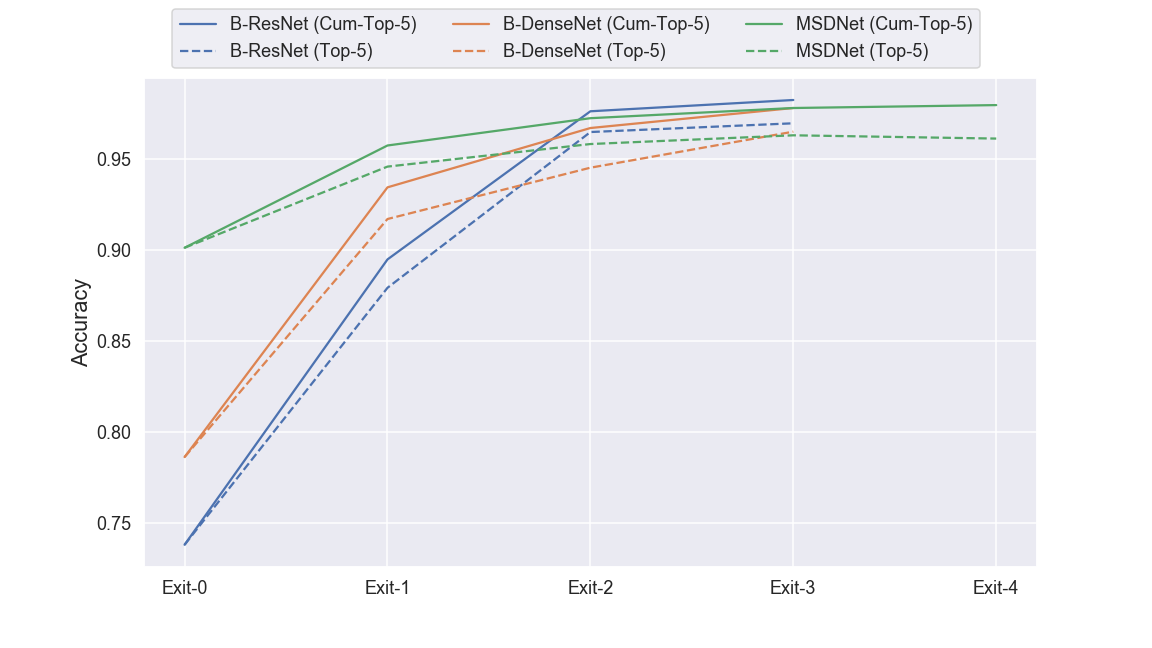
\includegraphics[width=\linewidth]{figures/edge/top5cumulative}
	\caption[Top-5 Cumulative]{Model Cumulative Top-5 Accuracy}
	\label{fig:top-5-cumulative}
\end{figure}

From the figure we can tell, that having multiple predictions does indeed improve the cumulative top-5. However, cherry-picking the correct prediction from the available predictions is not trivial. Figure \ref{} plots the results using the combination function defined in \ref{}. 

\begin{figure}
	\captionsetup[subfigure]{justification=centering}
	\centering
	
\includegraphics[width=.7\linewidth]{figures/edge/exit0-4_legend}
	\subfloat[B-ResNet]{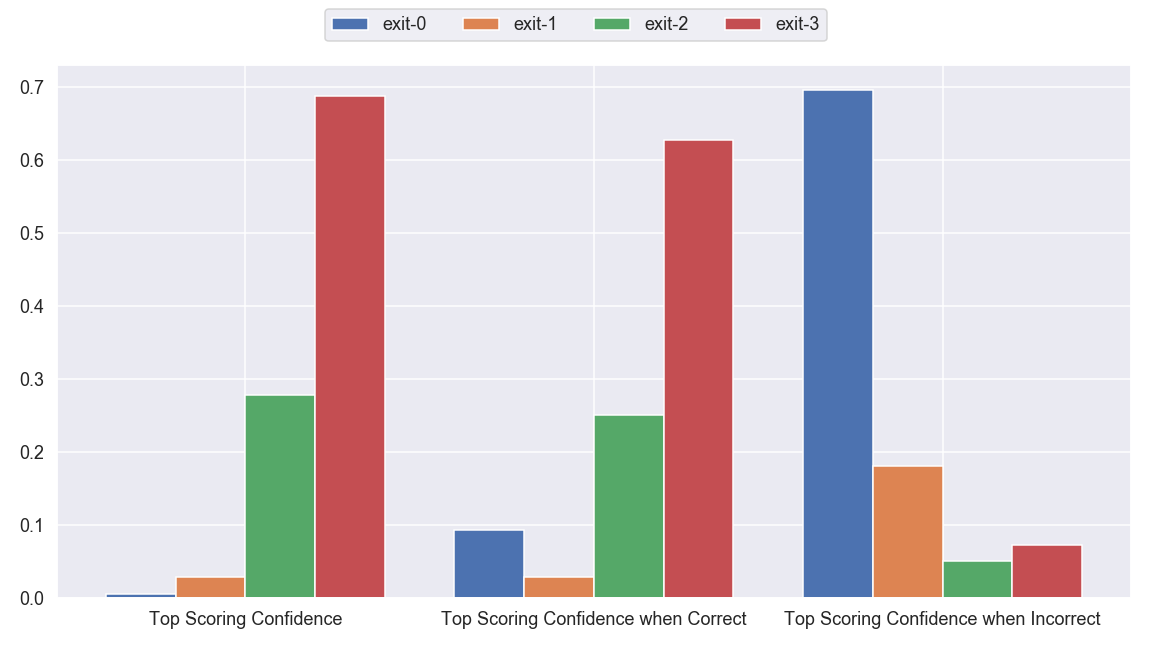
\includegraphics[width=.33\linewidth]{figures/edge/b-resnet_correctness}}
	\hfill
	\subfloat[B-DenseNet]{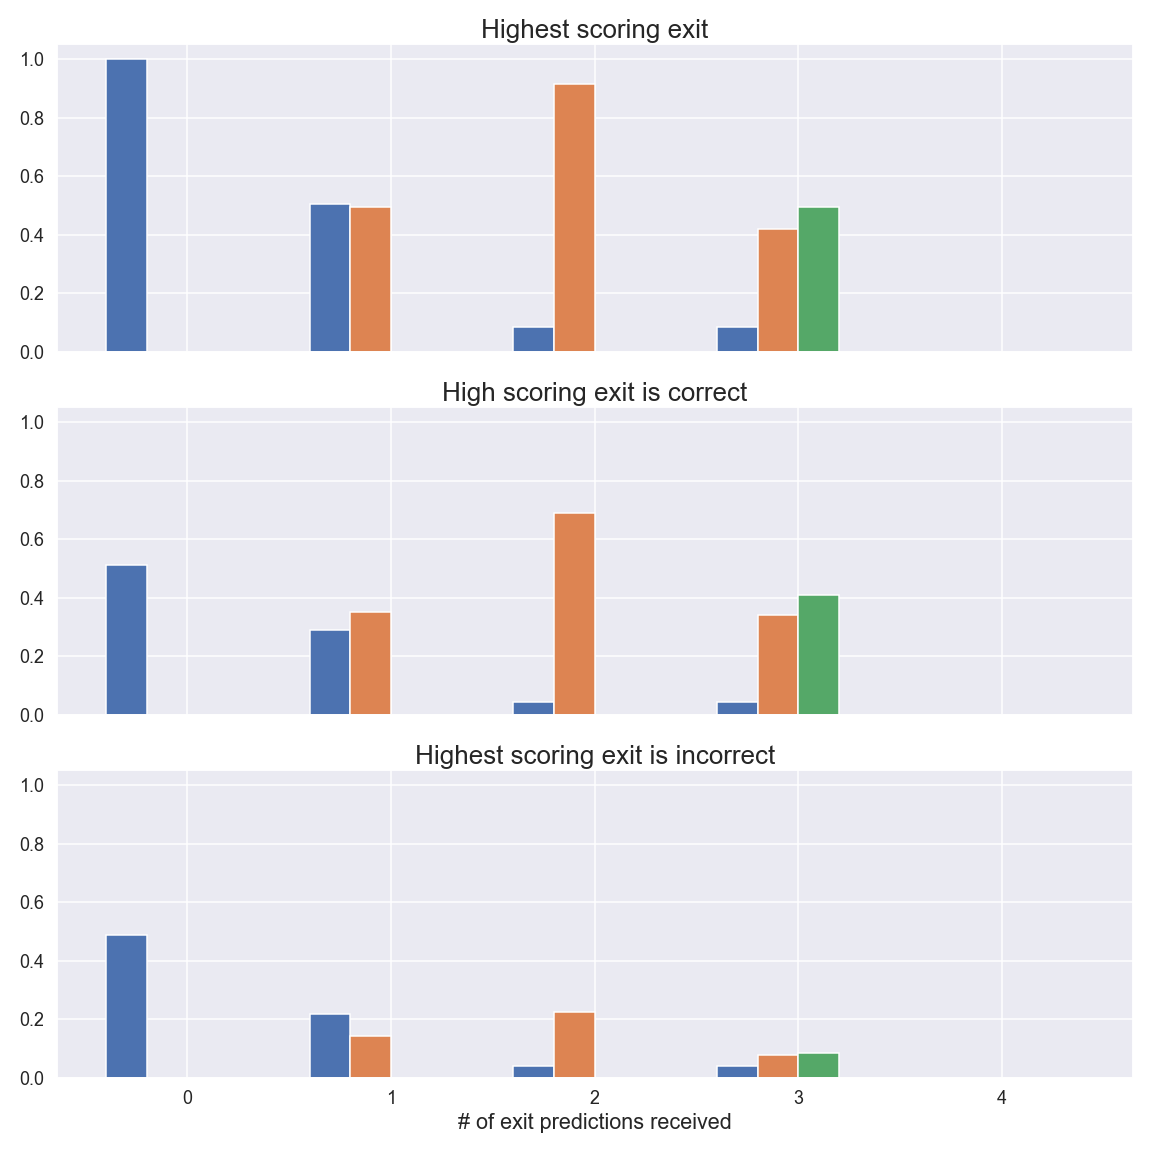
\includegraphics[width=.33\linewidth]{figures/edge/b-densenet_correctness}}
	\hfill
	\subfloat[MSDNet]{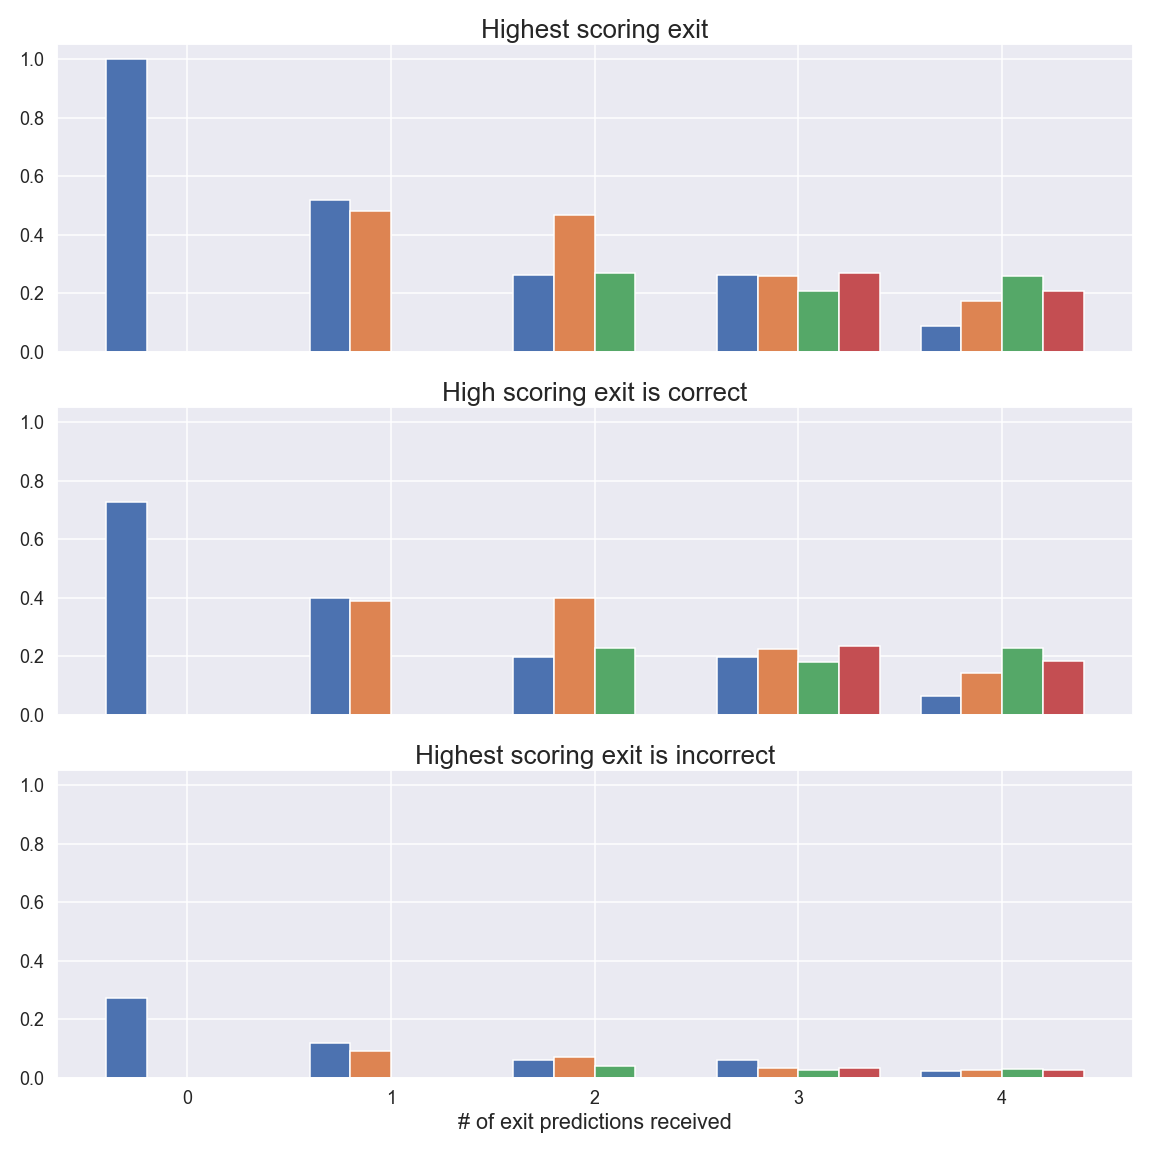
\includegraphics[width=.33\linewidth]{figures/edge/msdnet_correctness}}
	\caption[short text]{text}
	\label{fig:exit-highscore}
\end{figure}


Given this insight we define methods to combine the prediction information from multiple exit as efforts to improving the overall model accuracy. 

\subsection{Combining Prediction Information}


\begin{figure}
	\captionsetup[subfigure]{justification=centering,farskip=1pt,captionskip=1pt}
	\centering
	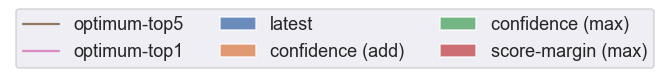
\includegraphics[width=.7\linewidth, keepaspectratio]{figures/edge/theoretical_score_combination_legend}
	\subfloat[subcaption]{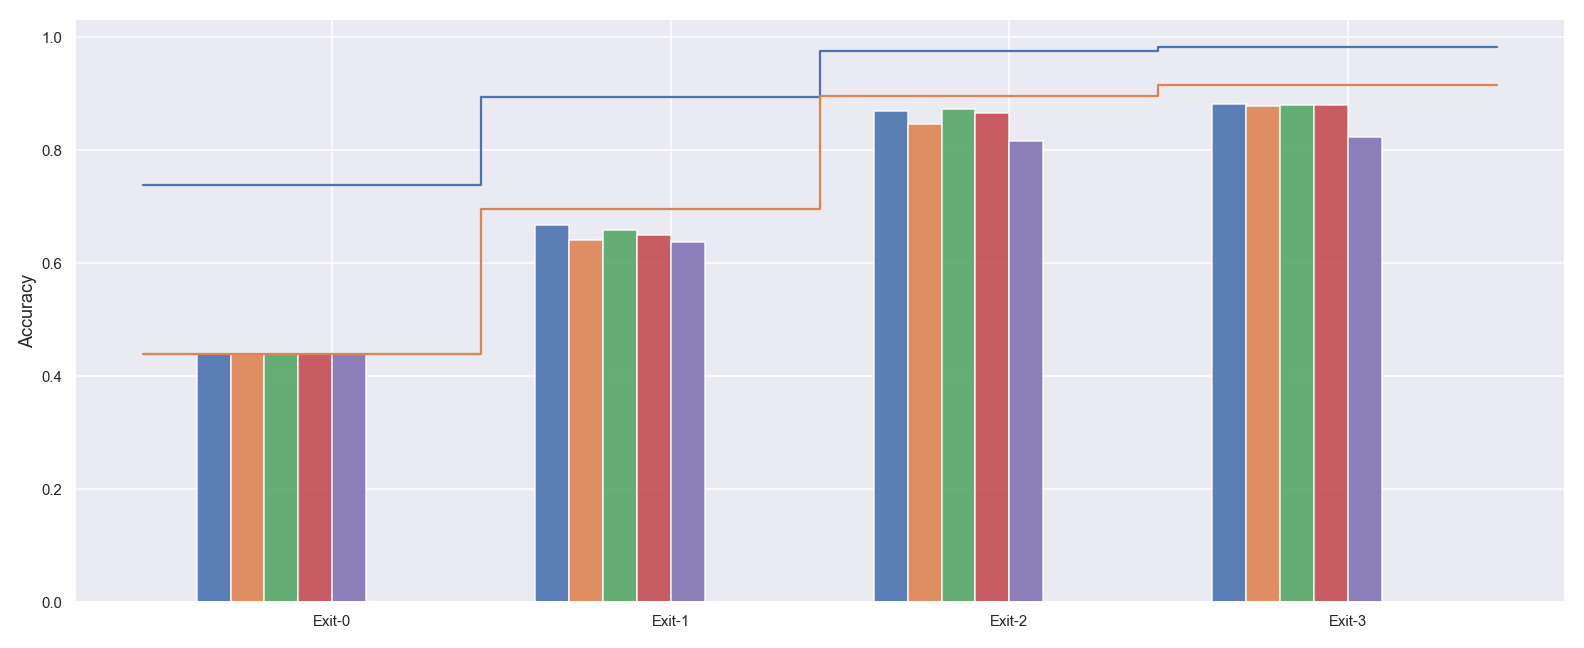
\includegraphics[height=.27\textheight, keepaspectratio]{figures/edge/b-resnet_theoretical_score_combinations}}
	\hfill
	\subfloat[subcaption]{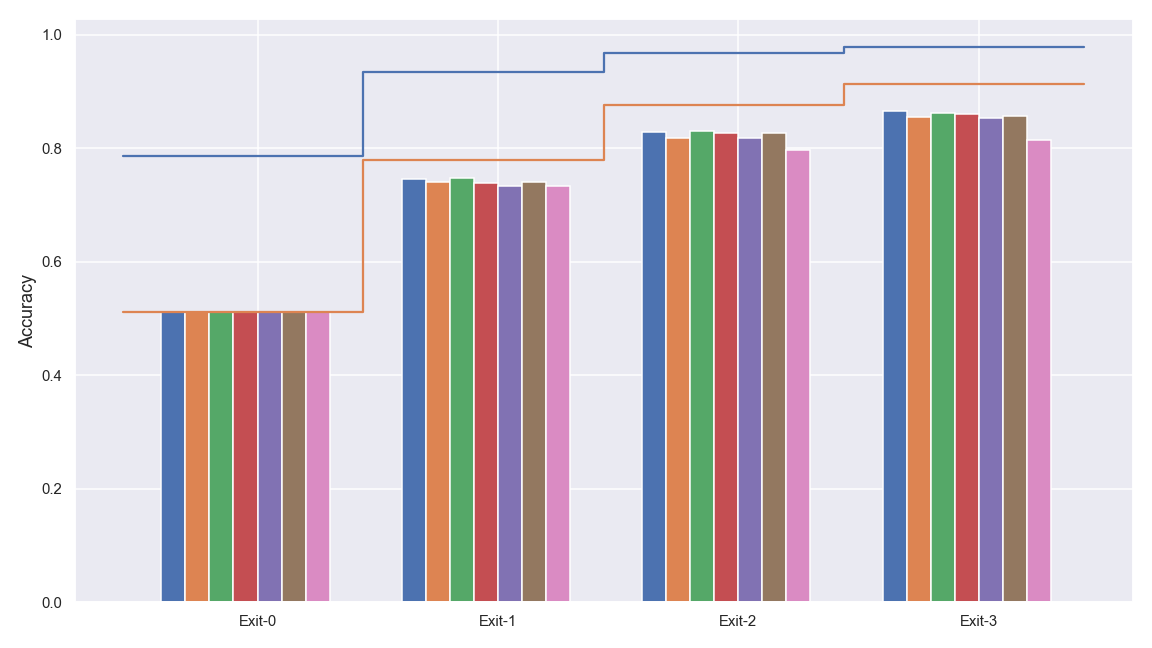
\includegraphics[height=.27\textheight, keepaspectratio]{figures/edge/b-densenet_theoretical_score_combinations}}
	\hfill
	\subfloat[subcaption]{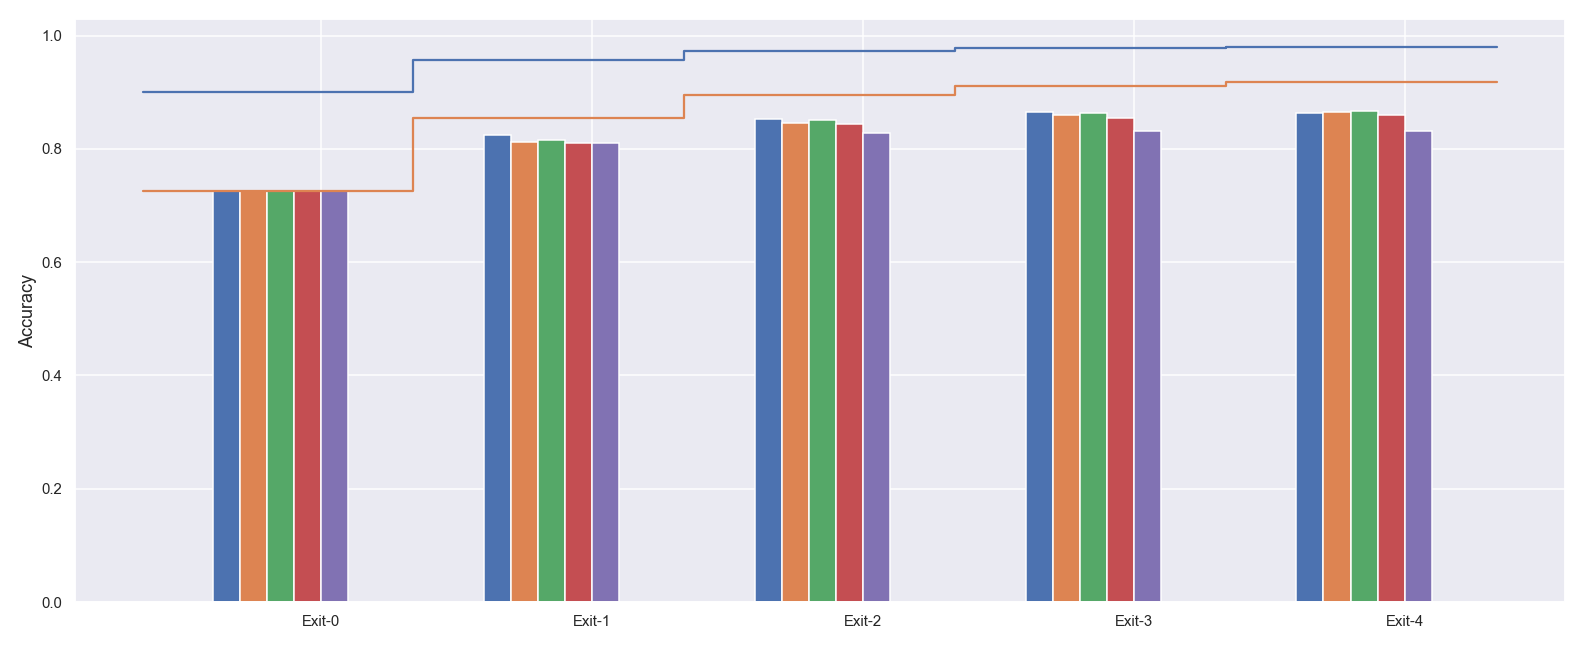
\includegraphics[height=.27\textheight, keepaspectratio]{figures/edge/msdnet_theoretical_score_combinations}}
	\caption[short text]{text}
	\label{fig:theoretical-info-combi}
\end{figure}

The blue line optimum-top5 show the maximum achievable accuracy, if we were always able to pick the right class among the top5 predictions given the number of exit results received. The orange line optimum-top1 show the optimal line if, we were always able to pick the correct class among the top1 prediction given the number exit results received.

\subsection{Delay Constraint}

How far are we able to in inference process under different time constraints? 

\todo{NB. I have not made MSDNet work on offloading the intermittent error still persists. I've brought it home to check if its a network error.}


\begin{figure}
	\captionsetup[subfigure]{justification=centering,farskip=1pt,captionskip=1pt}
	\centering
	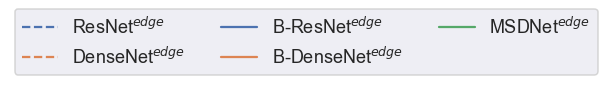
\includegraphics[width=.7\linewidth]{figures/edge/offloading_legend}
	\subfloat[]{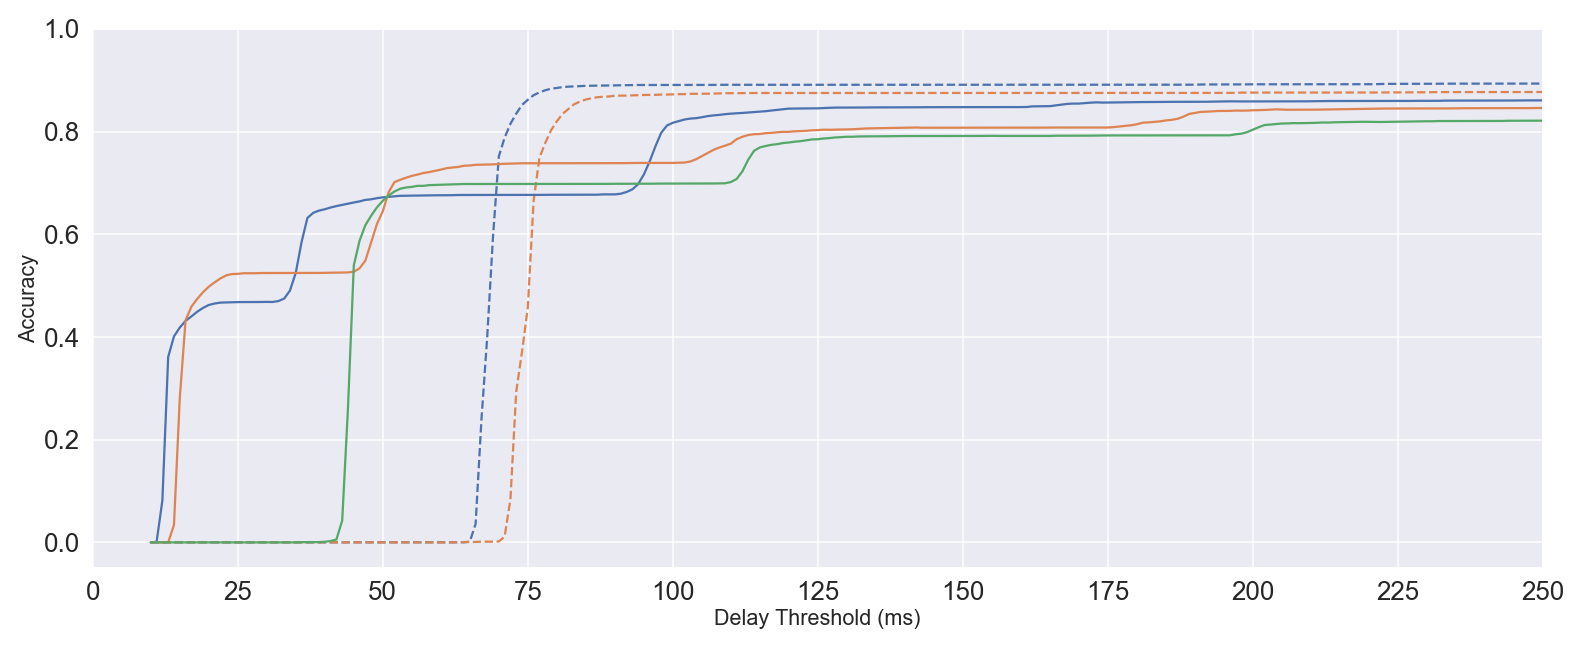
\includegraphics[width=\linewidth]{figures/edge/jetson_offloading}}
	\hfill
%	\subfloat[Local Jetson TX2]{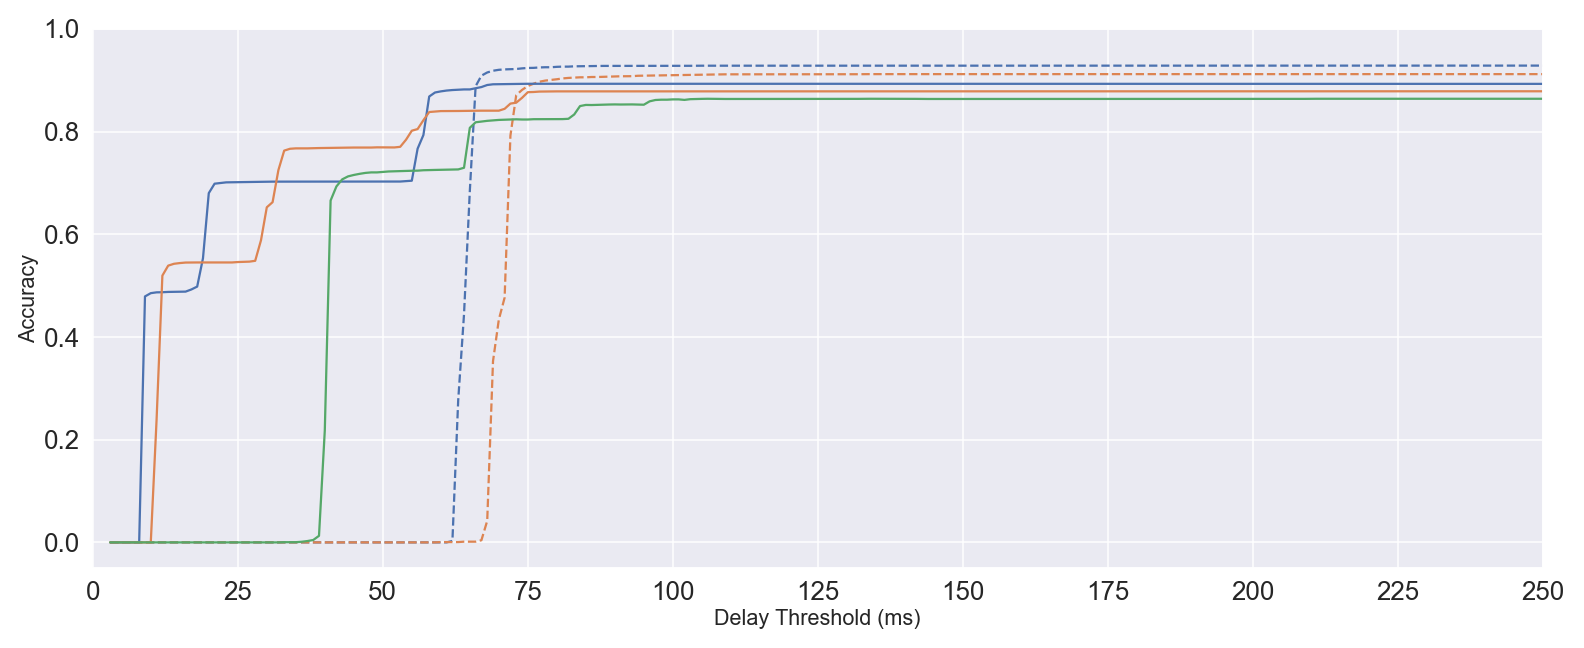
\includegraphics[width=\linewidth]{figures/delay_plots/jetson__delay_threshold}}
	\caption[short text]{text}
	\label{fig:practical-offloading}
\end{figure} \todo{should I compare these two?}


\begin{longtabu}{>{\bfseries}X|X|X|X|X}
	\caption[]{} \label{tbl:time-offloadinf} \\
	\toprule
	\rowfont{\bfseries}
	 & \multicolumn4{c}{Communication Time (ms)}    \tabularnewline
	 \tabucline{2-5}
	\rowfont{\bfseries} Offloading & Mean & Std. & Min & Max   \tabularnewline
	\bottomrule
	\endfirsthead
	\multicolumn{3}{@{}l}{\textbf{\textcolor{black}{Table \ref{}:}} continued}\\
	\toprule
	\rowfont{\bfseries}
	Offloading & Up- and downlink Communication Time (ms) &    \tabularnewline
	\bottomrule
	\endhead % all the lines above this will be repeated on every page
	\bottomrule
	\multicolumn{3}{@{}l}{continued \ldots}\\
	\endfoot
	\hline
	\endlastfoot
	NUC to Jetson	& 25.68	& 110.93 & 2.35 & 962.76  \tabularnewline
									
	\bottomrule
\end{longtabu}
Should I create hybrid combinations? Maybe only combine info from exit-0 and -1 and always let exit-2 and -3 have the final say if available? What if we can combine info from those two and omit the poor ones? 

\begin{figure}
	\captionsetup[subfigure]{justification=centering, farskip=0pt,captionskip=0pt}
	\centering
	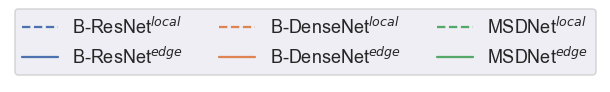
\includegraphics[height=.05\textheight]{figures/edge/offloading_vs_local_legend}
	\hfill
	\subfloat[B-ResNet]{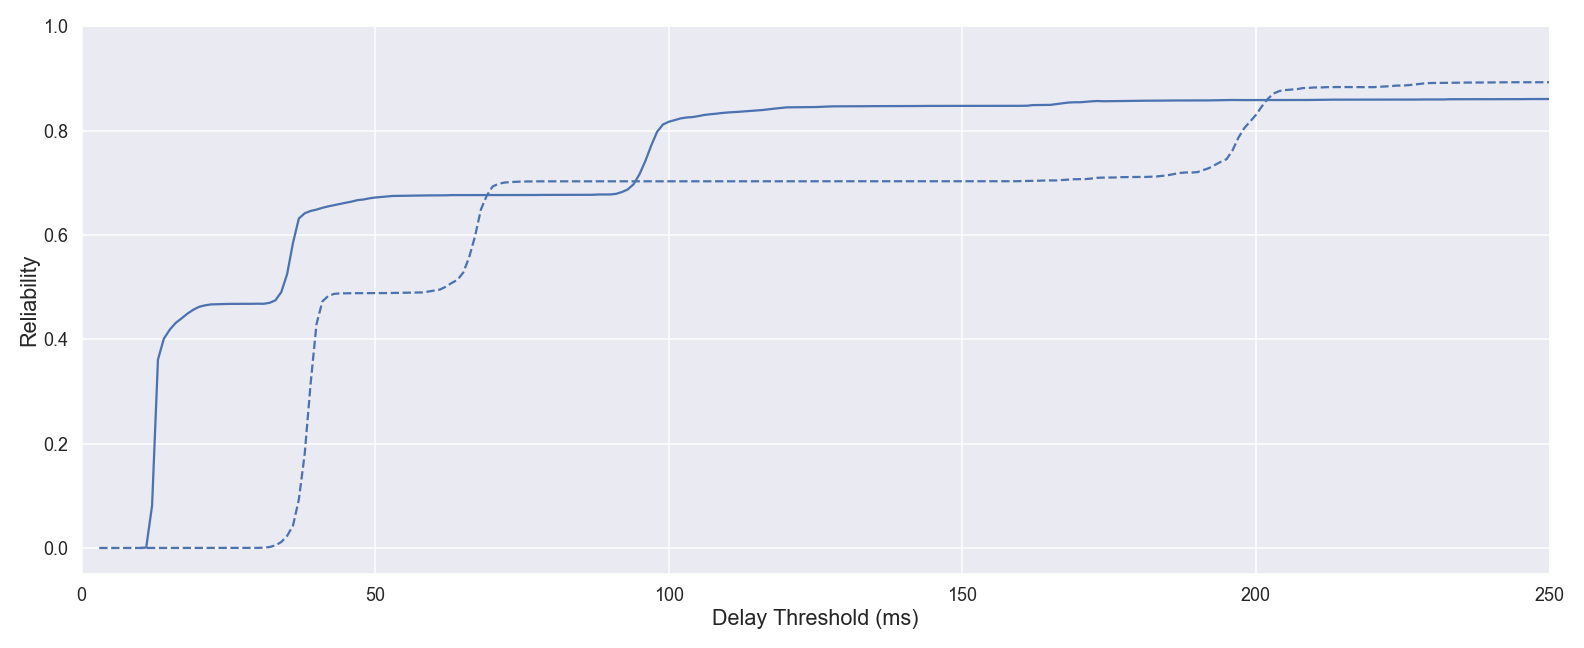
\includegraphics[width=\textwidth,height=.29\textheight,keepaspectratio]{figures/edge/b-resnet_offloading_vs_local}}
	\hfill
	\subfloat[B-DenseNet]{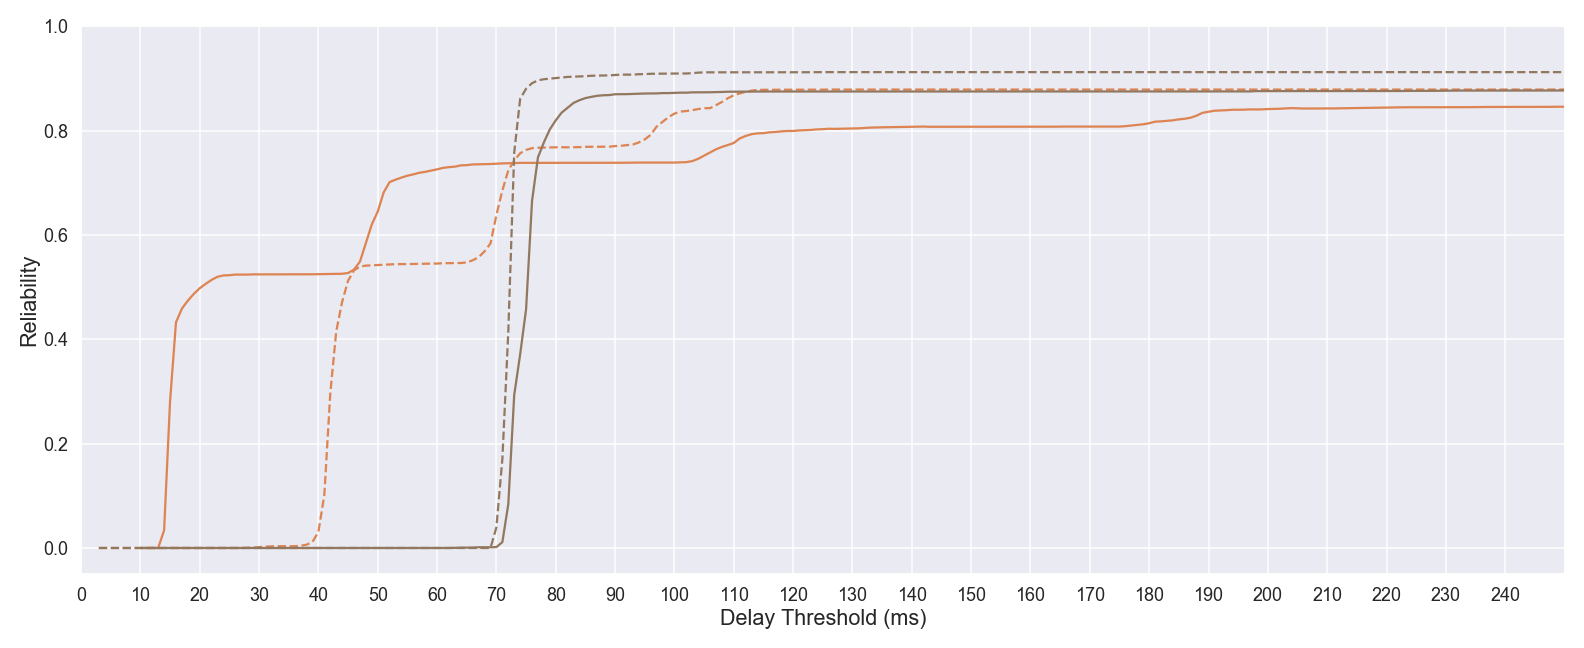
\includegraphics[width=\textwidth,height=.29\textheight,keepaspectratio]{figures/edge/b-densenet_offloading_vs_local}}
	\hfill
	\subfloat[MSDNet]{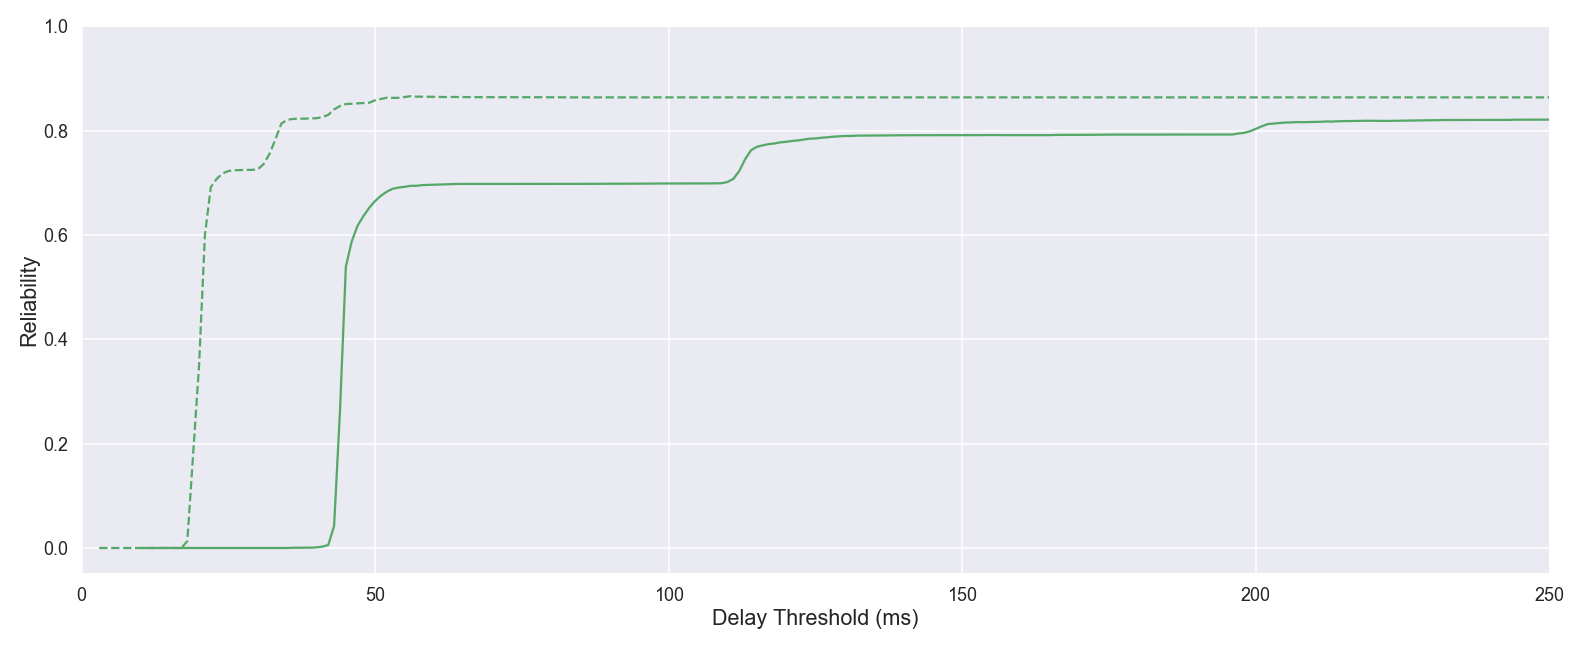
\includegraphics[width=\textwidth,height=.29\textheight,keepaspectratio]{figures/edge/msdnet_offloading_vs_local}}
	\caption[Offloading Jetson vs. Local NUC]{Offloading inference to Jetson vs. Local inference on NUC}
	\label{fig:offloading-vs-local}
\end{figure}


\subsection{Transport Protocol} 

Offloading tasks over the network, irregardless fully or partially requires a transport protocol. The selection is typically a choice of either \gls{tcp} or \gls{udp}. \gls{tcp} is a reliable protocol, that guarantee no losses by retransmission of lost packets. \gls{udp} on the other hand is a best-effort protocol, that accept packets loss, thus not introducing retransmission communication overhead. 


Fully offloading \gls{jpeg} compressed images for classification require no losses for human-readability. Sending intermediate features of a \gls{dnn} may not be as intolerant to losses and might be able to function with the far more lightweight \gls{udp}. In current research literature the choice of \gls{tcp} seems given in advance.  

In this experiment the \gls{tcp} transmission time and retransmission rate is investigated under different communication environments. 

\begin{figure}
	\centering
	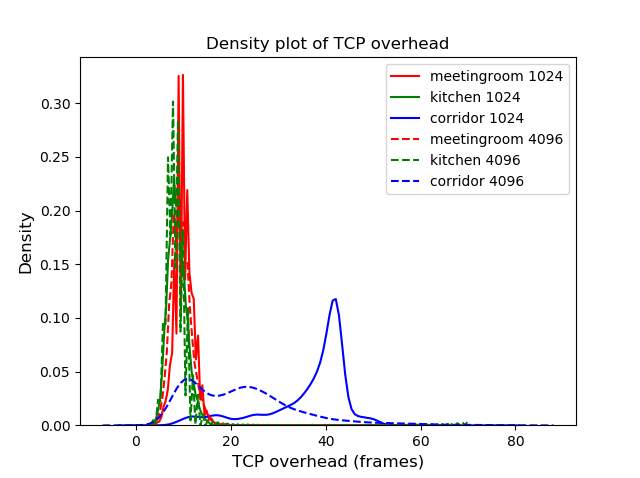
\includegraphics[width=\linewidth]{figures/tcp/tcpoverhead}
	\caption[TCP retransmission overhead]{TCP retransmission overhead}
\end{figure}

\section{Summary}

Edgent: The selection of exit is based on distributions of inference time, this introduces some uncertainty, as not all samples might be able to meet the latency requirement, this can be caused be derivation in compute time, congestions in the network latency or server workload. One key feature of early exiting is the ability to obtain intermediate predictions, this allow for parallel execution while offloading. The end-device might only be able to reach an early exit within the time frame, where edge server reaches a later one. However, unexpectedly no reply is received by the end-device within the time frame, then the application can use the local obtained prediction from an earlier exit. 

Or a collaborative scheme might be used, where the end-device locally processes the algorithm up to an early exit and obtains a prediction, then it offload the rest of the execution in a cascaded manner for remote execution, still if no reply is received by the end-device within the time frame a locally obtained prediction is available albeit less reliable than if the remote prediction would have arrived in time. 

All offloading can lead to lost predictions under time stringent time constraints. If local processing is possible, then;

\begin{enumdescript}
	\item[Collaborative Edge] where local inference of an early exit \gls{dnn} up to the first exit and then offload to the edge for remaining inference. The upside is, that running locally up to an exit, that should always be achievable guarantee a single prediction is available and mitigates lost prediction. The downsides are wasted idle time on edge server, as the slower end-device must do the most demanding early layers of the \gls{dnn}. Additionally offloading intermediate features that are typically larger than the original compressed images, hence the overall time becomes worse as communication is the bottleneck. This collaborative scheme require sophisticated compression of intermediate feature as in \cite{choi_near-lossless_2018} or a using \gls{bottlenet} layers.
	\item[Big/Little] A modified version of the Big/Little \gls{dnn}, where the end device offloads the compressed image to edge server and in parallel process a smaller and less accurate \gls{dnn} locally. The upside is, that the application can then always use the locally obtained prediction and choose to discard it as more accurate prediction arrives or combine information local and incoming predictions.
\end{enumdescript}

